\documentclass[12pt, twoside]{article}
\usepackage[letterpaper, margin=1in, headsep=0.5in]{geometry}
\usepackage[english]{babel}
\usepackage[utf8]{inputenc}
\usepackage{amsmath}
\usepackage{amsfonts}
\usepackage{amssymb}
\usepackage{tikz}
%\usetikzlibrary{quotes, angles}

\usepackage{graphicx}
\usepackage{enumitem}
\usepackage{multicol}

\usepackage{fancyhdr}
\pagestyle{fancy}
\fancyhf{}
\renewcommand{\headrulewidth}{0pt} % disable the underline of the header

\fancyhead[LE]{\thepage}
\fancyhead[RO]{\thepage \\ Name: \hspace{4cm} \,\\}
\fancyhead[LO]{BECA / Dr. Huson / Geometry\\* Unit 7: Similarity\\* 2 January 2020}

\begin{document}
\subsubsection*{7.1 Homework: Similar triangles, dilations}
  \begin{enumerate}

    \item Given $\triangle ABC \sim \triangle ADE$ with sides $AC = 7$, $BC = 4$, $AB = 8$, and of $DE = 10$ find the scale factor $k$ and the lengths $AD$ and $AE$. Then find $CE$ and $BD$. %\vspace{1cm}
    \begin{multicols}{2}
      \begin{enumerate}
        \item $k=$ \vspace{0.3cm}
        \item $AD=$ \vspace{0.3cm}
        \item $AE=$ \vspace{0.3cm}
        \item $CE=$
        \item $BD=$
      \end{enumerate}
      \begin{flushright}
        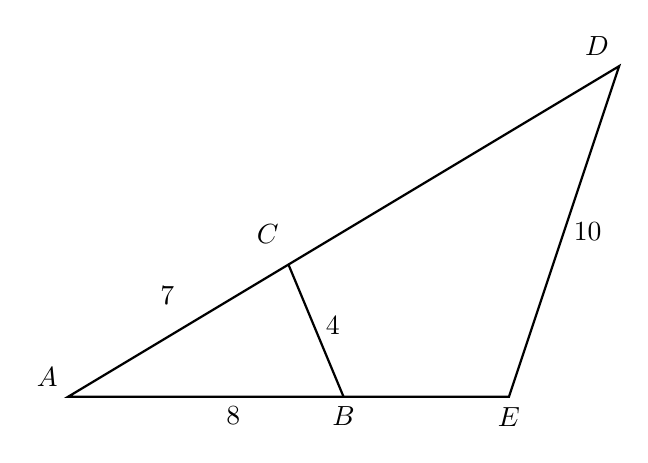
\begin{tikzpicture}[scale=0.7]
          \draw [-, thick] (0,0) node[above left]{$A$}--
          (8,0) node[below]{$E$}--
          (10,6) node[above left]{$D$}--cycle;
          \draw [thick] (5,0)--(4,2.4);
          \node at (5,0) [below]{$B$};
          \node at (4,2.6) [above left]{$C$};
          \node at (3, 0) [below]{$8$};
          \node at (1.8,1.5) [above]{$7$};
          \node at (9, 3) [right]{$10$};
          \node at (4.5, 1.3) [right]{$4$}; \vspace{1cm}
        \end{tikzpicture}
      \end{flushright} 
    \end{multicols}%\vspace{1.5cm}

  \item After a dilation centered at the origin, the image of $\overline{AB}$ is $\overline{A'B'}$. If the coordinates of the endpoints of these segments are $A(-1,-3)$, $B(4,-5)$, $A'(-2,-6)$, and $B'(8,-10)$, find the scale factor of the dilation.\\[0.25cm]
  Make a table of coordinate pairs and graph the two line segments,  $\overline{AB}$ and  $\overline{A'B'}$, on the set of axes below.
    \begin{flushright}
      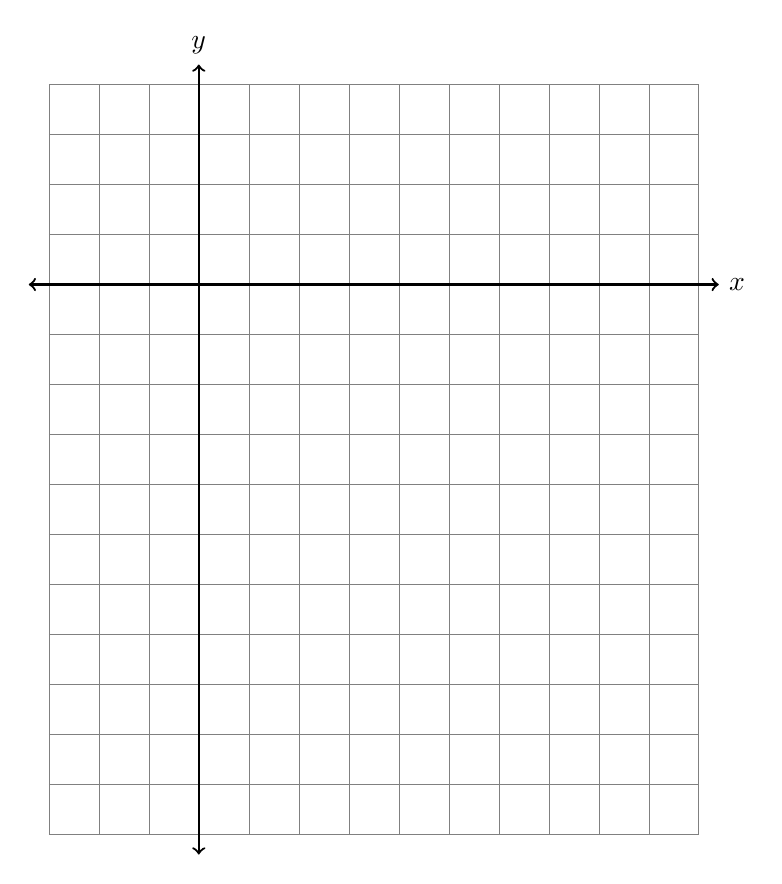
\begin{tikzpicture}[scale=.635]
        \draw [help lines] (-3,-11) grid (10,4);
        \draw [thick, <->] (-3.4,0) -- (10.4,0) node [right] {$x$};
        \draw [thick, <->] (0,-11.4)--(0,4.4) node [above] {$y$};
      \end{tikzpicture}
    \end{flushright}



\newpage
  \item Given $\triangle ABP \sim \triangle JKP$ as shown below. $AB=9.6$, $AP=12.0$, $BP=6.3$, and $JK=14.4$. Find $JP$.
  \begin{flushright}
  \begin{tikzpicture}[scale=1.4]
      \draw [thick]
        (-0.25,-1)node[below left]{$B$}--
        (0.5,2)node[left]{$K$}--
        (4,0)node[below left]{$J$}--
        (0,0)node[above left]{$P$}--
        (-2,0)node[left]{$A$}--cycle;
    \end{tikzpicture}
    \end{flushright}
    \vspace{2cm}

  \item In the diagram below of $\triangle ABC$, $D$ is a point on $\overline{BA}$, $E$ is a point on $\overline{BC}$, and $\overline{DE}$ is drawn. \\*[2pt] 
  If $BD=5$, $DA=12$, and $BE=7$, what is the length of $\overline{BC}$ so that $\overline{AC} \parallel \overline{DE}$?
  \begin{flushright}
      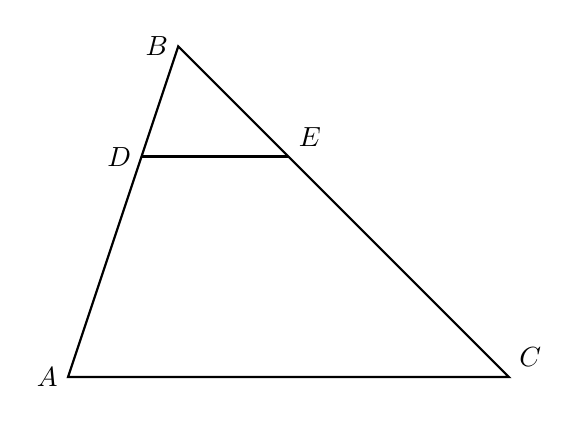
\begin{tikzpicture}[scale=0.7]
        \draw [thick]
        (0,0)node[left]{$A$}--
        (8,0)node[above right]{$C$}--
        (2,6)node[left]{$B$}--cycle;
        \draw [thick]
        (4/3,4)node[left]{$D$}--
        (4,4)node[above right]{$E$};
      \end{tikzpicture}
    \end{flushright}

\end{enumerate}
\end{document}